\chapter{Search Strategy}
\label{ch:SearchStrategy}

\section{Physics Objects}\label{PhysObj}
There are many different types of physics objects that we are interested in when working with particle physics experiments. Since these particles have very short lifetimes, $\mathcal{O}(\text{decay})=10^{-23}$ s, we mainly interact with the decay products of the event, such as, jets $(N_j)$, heavy object tagging $(\nb, \nt, \nw, \nrt)$, missing transverse momentum (\met), scalar sum jet momentum $(H_T)$, soft-b tagging, denoted as $\nsv$, transverse mass between tagged $b$ quarks and \met{} $(m_T(b_{1,2}, \met))$, Initial State Radiation, and lepton identification. We will look into each of these objects further in this chapter.

\subsection{Jets}\label{Jets}
In an interaction whenever a quark is made it comes in pairs $(q\overline{q})$ such that the total color charge of the interaction is neutral. Typically due to conservation of momentum the quarks may originally be produced near the interaction point but will quickly start to move away from each other. Eventually the quarks will move far enough apart and will have enough potential energy in the gluon connections between them that it is then more efficient to create a new quark-antiquark $(q\overline{q})$ pair. This will continue to occur in a sequence of radiating gluons and the production of pairs of charged particles, see Fig. \ref{JetHadronization}. In the final state, the energy deposited in the HCAL is a cluster of charged particles of a radius, $\Delta R=\sqrt{\Delta\eta^2+\Delta\phi^2}$. There are many algorithms to reconstruct the jets which must satisfy the requirements in Ref. \cite{noauthor_jet_2010}. We are mainly interested in the anti-kT Jet algorithm \cite{cacciari_anti-ktjet_2008} method which uses the transverse momentum of the particles within a certain radius $\Delta R = 0.4 (0.8)$ for AK4(AK8) jets \cite{noauthor_https://twiki.cern.ch/twiki/bin/view/cms/jetid_nodate, noauthor_https://twiki.cern.ch/twiki/bin/view/cms/introtojec_nodate}. A charged hadron subtraction is also used to correct for the pileup, the number of collisions seen during a single proton beam crossing \cite{cacciari_pileup_2008, noauthor_pileup_2014}. For AK8 jets the pileup contribution is accounted for using the "pileup per particle identification" method \cite{bertolini_pileup_2014, noauthor_pileup_2014}, where each particle is weighted by its probability of originating from the primary vertex. Once the jets have been identified, we can analyze their respective properties to determine the likelihood of the particle it originated from, such as a $b, t,$ or \W. 

\begin{figure}
 	\centering
	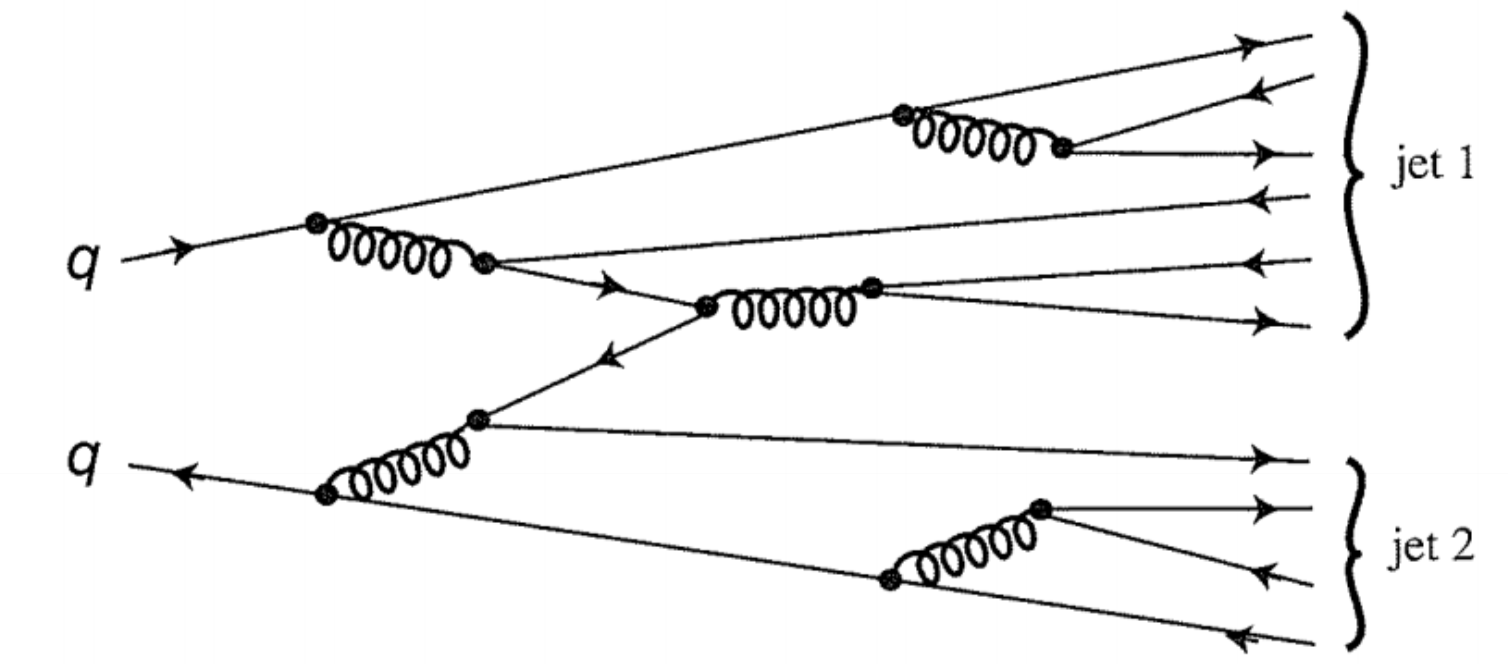
\includegraphics[width=0.75\textwidth]{JetHadronization.png}
 	\caption[Jet Hadronization]{A diagram of a quark pair radiating gluons that decay into more quark pairs in a process called hadronization \cite{griffiths_introduction_2008}.}
 	\label{JetHadronization} 
\end{figure}

\subsection{Heavy Object Tagging}\label{HeavyObject}
Since this search is looking for a massive particle which then decays to slightly less massive particles we need to be able to identify and distinguish between them. We use various algorithms and neural networks to identify jets from $b$ quarks, $t$ quarks, or from \W {} bosons. 

\subsubsection{B-Tagging}\label{Btagging}
Firstly, \B-tagged jets are jets that are likely to have originated from a \B{} quark. For \B{} quarks with large transverse momentum, we use a Deep Combined Secondary Vertex (DeepCSV) algorithm that involves neural networks\cite{noauthor_performance_nodate}. The medium working point recommended by the B-tag POG, corresponding to a threshold of 0.6324 0.4941, and 0.4184 for the 2016, 2017, and 2018 eras, respectively \cite{noauthor_https://twiki.cern.ch/twiki/bin/viewauth/cms/btagrecommendation2016legacy_nodate, noauthor_https://twiki.cern.ch/twiki/bin/viewauth/cms/btagrecommendation94x_nodate, noauthor_https://twiki.cern.ch/twiki/bin/viewauth/cms/btagrecommendation102x_nodate, noauthor_https://twiki.cern.ch/twiki/bin/viewauth/cms/btagsfmethods_nodate}. The medium working point is defined such that the percentage of a light jet being misidentified as a \bjet{} is 1\%.

\begin{figure}
 	\centering
	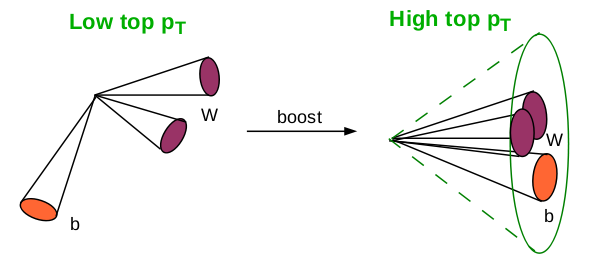
\includegraphics[width=0.75\textwidth]{TopDecayBoost.png}
 	\caption[Top Decays]{The two types of top quark reconstructions, when each decay product is easily identifiable (resolved) or when the particles are close together (boosted).}
 	\label{TopDecays} 
\end{figure}

\subsubsection{Top/W Tagging}\label{TopTagging}
Top quark tagging is an essential part of our analysis. The top quark tagging algorithm is designed to have a high reconstruction efficiency for entire \pt{} spectrum of the top quark in our signal models. The anti-kt algorithm using a distance parameter, $\Delta R=0.8$, is expected to contain the energy clusters of all of the decay product of boosted $t$ quarks \cite{noauthor_top_nodate, noauthor_identification_nodate-1}, see Fig. \ref{TopDecays}, with $\pt>300$ \GeV{} or \W{} bosons with $\pt>200$ \GeV. These decays are reminiscent of the expected decay, $t\rightarrow bq\bar{q}^\prime$, when it is a highly Lorentz boosted $t$ quark decay. The requirements are:
\begin{itemize}
	\item Medium working point $>0.937, 0.895, 0.895 (0.973, 0.991, 0.991)$ for boosted $t$ $(W)$ for the separate 2016, 2017, and 2018 eras, respectively.
	\item Reconstructed soft drop\cite{larkoski_soft_2014, dasgupta_towards_2013} mass: $105<m_t<210$ \GeV{} and $65<m_W<105$ \GeV.
	\item Boosted tops: $\pt=300$ \GeV, $|\eta|<2.0$ and $W$: $\pt=200$ \GeV, $|\eta|<2.0$.
\end{itemize}

There is another type of top that can be reconstructed, which is when each subjet of the top decay can be resolved into each individual jet, denoted as a resolved top, see Fig. \ref{TopDecays}. The requirements are:
\begin{itemize}
	\item Medium working point: 0.92 for all eras.
	\item $|\eta(j_{1,2,3})|<2.4$ and $b$-tag discriminator: $>0.6324, 0.4941, 0.4184$ for the separate 2016, 2017, and 2018 eras, respectively. The number of jets in the event that pass these cuts should be $\geq2$.
\end{itemize}
These object definitions, \nt, \nw, \nrt, are orthogonal to each other and are used to bin our search and control regions. 

\subsection{Missing Transverse Momentum}\label{MET}
The missing transverse momentum \cite{lester_measuring_1999, barr_variable_2003} is the negative vector sum of the total transverse momentum measured in the detector,
\begin{equation}
\met=-\sum_{i\in\text{vis}}\overrightarrow{p}_{i, T},
\end{equation}
where the momentum runs over every visible (vis) particle in the event. Ideally, if the detector was $100\%$ efficient this quantity would always be zero due to conservation of momentum, but many things, such as detector efficiency, particles that are weakly interacting, or particles beyond the SM will cause the missing energy. Because of these, \met{} is a good discriminator for searching for physics beyond the SM \cite{noauthor_https://twiki.cern.ch/twiki/bin/view/cms/missingetrun2corrections_nodate}. 

%\subsection{MET Filters}
%Need to add MET Filters here.

\subsection{$H_T$}\label{HT}
Another interesting quantity is $H_T$, which is the scalar sum of the \pt{} of all of the jets in an event,
\begin{equation}
H_T=\sum_{i\in\text{jets}}p_{i,T}.
\end{equation}
This quantity is quite useful when trying to identify massive particles and is quite good at suppressing QCD multijet background.

\subsection{Soft $b$-Tagging}\label{SV}

The ability to identify secondary vertices is essential in searches for the top squark, see Sec. \ref{sec:Production}. Since the b quark is a long lived particle, about $10^{-12}$ seconds, it will travel many millimeters before decaying into other particles. A \B{} quark is identified during reconstruction, where the jet originating from a point separated from the primary vertex $(PV)$, known as the secondary vertex $(SV)$. The displaced vertex of the long lived $b$ quark with low \pt{} has many interesting kinematic properties that we can use to identify them, known as soft $b$-tagging. 

\begin{figure}
 	\centering
	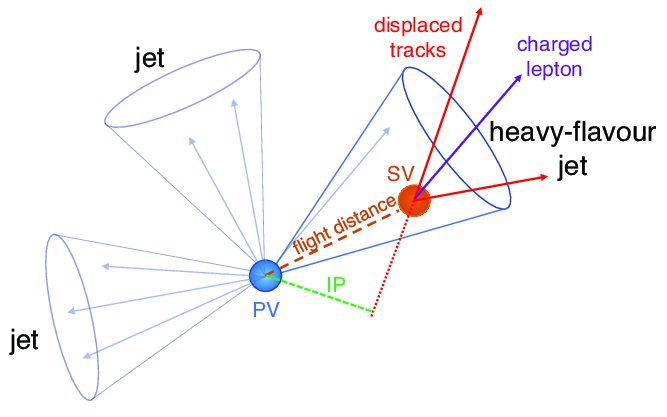
\includegraphics[width=0.75\textwidth]{SecondaryVertex.png}
 	\caption[Secondary Vertex Diagram]{An interaction that produces a long lived particle that has a reconstructed SV.}
 	\label{SecondaryVertex} 
\end{figure}

This search also targets models that produce very soft bottom or charm quarks. A large fraction of events contain b quarks with \pt{} below the 20 GeV jet threshold which may fail to be reconstructed as jets or become b-tagged. Identification of these soft quarks improves our ability to separate potential signal events from the SM background. We therefore aim to identify $b$ or $c$ quarks based on the presence of a SV reconstructed using the Inclusive Vertex Finder (IVF) \cite{noauthor_https://twiki.cern.ch/twiki/bin/view/main/inclusivesecondaryvertexfinder_nodate, fruehwirth_new_2003}. Additional requirements on the SV observable are applied to suppress the background originating from light quarks. These selected SV may be referred to as soft $b$-tags and are constructed to be orthogonal to the jets and b-tagged jets used in this analysis. 

The requirements on each SV to pass the soft b-tagging definition are:
\begin{itemize}
	 \item The distance in the transverse plane between the SV and the PV $\leq3$ cm.
	 \item The significance of the distance, SIP3D, between the SV and the PV $\geq4$.
	 \item The pointing angle, defined as $\cos(\overrightarrow{PV,SV},\overrightarrow{p_{SV}})\geq0.98$, where $\overrightarrow{p_{SV}}$ is the total four-momentum of the tracks associated with the SV. 
	 \item The number of tracks associated with the SV is greater or equal to 3.
	 \item The \pt{} of the SV is less than 20 GeV.
\end{itemize}
Identification of soft b-quarks is necessary for potential signal region where the stop does not directly decay into a top quark and is essential for some of our search region bins. 

\subsection{Transverse Energy between $b$ quarks and \met}
We will end up dividing the search regions we are interested in into two different groups. They will be distinguished by a parameter known as the transverse mass between the leading \bjet{} and \met{} defined as:
\begin{equation}\label{TransverseMass}
\mtb=\sqrt{2\cdot\met\cdot\pt(b)(1-\cos(\slashed{E}_\phi,p_{\phi}(b)))},
\end{equation}
where \pt(b) is the momentum of the leading \bjet{} and $\slashed{E}_\phi$ and $p_{\phi}(b)$ is the $\phi$ component of the missing energy and \bjet{}, respectively. This will be used to distinguish between our low and high mass search regions, see Section \ref{SearchRegions}.


\subsection{Initial-state Radiation}\label{ISRpt}

Initial-state radiation (ISR) may be clustered into one of the large-$R$ jets clustered with a distance parameter, $\Delta R=0.8$. We use the larger radius jets to be sensitive to ISR with gluon splitting, when a jet radiates a gluon that pair produces two quarks. The ISR jet is identified as being the hardest of the large-$R$ jets with $\pt>200$ GeV which fails the loose b-tagging working point and is not identified as a top or W. This is a good parameter for jets that are neither tagged as $t$ or \W{} in the low \dm{} region of our search.
 
 \subsection{Electron and Muon Identification}\label{EleMuonID}
 There are two sets of selection criteria used in the analysis for electrons \cite{noauthor_performance_2015} and muons \cite{collaboration_performance_2013}. The set of criteria used to efficiently reject events with an isolated electron is done with a "Veto" ID. An electron with a Veto ID must pass the following cuts:
 \begin{itemize}
	 \item $|\Delta\eta|<0.007(0.01),|\Delta\phi|<0.8(0.7)$ for the electrons (muons).
	 \item $\sigma_{i\eta i\eta}<0.01(0.03)$ for the electrons (muons).
	 \item $H/E<0.15(N/A)$.
	 \item $\text{PF isolation}/\pt(\text{cone } \Delta R=0.3)<0.15(0.15)$ for the electrons (muons).
	 \item $|d_{0}|<0.04(0.04),|d_Z|<0.2(0.2)$ for the electrons (muons).
 \end{itemize}
 for the barrel and endcap regions of the detector, where $H/E$ is the ratio of hadronic energy over electromagnetic energy. This veto ID is chosen such that the search region is most likely to be devoid of electrons, since it has a 95\% efficiency \cite{noauthor_https://twiki.cern.ch/twiki/bin/view/cms/cutbasedelectronidentificationrun2_nodate}.
 
 We use the Loose muon definition recommended by the Muon POG for the purposes of the muon veto \cite{noauthor_https://twiki.cern.ch/twiki/bin/view/cmspublic/swguidemuonidloose_muon_nodate}. A Loose muon is identified as a Particle Flow (PF)\cite{noauthor_cms_nodate} muon and can be either a global muon or an arbitrated tracker muon. Only candidates with transverse (longitudinal) impact parameter $|d_0|<0.2$ cm $(|d_z|<0.5 \text{cm},)$ with respect to the primary vertex, are considered. The electron and muon IDs are used in the definition of the Lost Lepton background which will be expanded upon further in Section \ref{sec:LL}. 
 
\subsection{Tau Identification}\label{TauID}
The Tau ID has been studied extensively in tests which looked into the custom MVA \cite{roe_boosted_2004, hoecker_tmva_2007, bravo_search_2015} similar to the one used in Ref. \cite{cms_collaboration_search_2016}, a cut-based IsoTrack method, and Tau POG MVA method of identifying hadronically decaying taus. The methods which provide the best improvement to the efficiency of identifying taus with a small fake rate is the combination of IsoTrack and Tau POG MVA. With the inclusion of the combined method for identifying hadronically decaying taus, the veto percentage is $\approx29.0\%(7.2\%)$ with an efficiency of the veto of $\approx49.1\%(22.6\%)$ for SM background (signal), see Appendix. \ref{sec:TauMVA}. 

For the IsoTrack method we require the following:
\begin{itemize}
	\item $\pt\geq5(10) \GeV, \text{iso}\leq0.2(0.1)$ for electrons and muons(pions);
	\item $m_T(\text{IsoTrack},\met)<100 \GeV$;
\end{itemize}
where $m_T(\text{IsoTrack},\met)$ is the transverse mass between the IsoTrack and \met. For the Tau POG method we require:
\begin{itemize}
	\item $\pt\geq20 \GeV, |\eta|<2.4$;
	\item idDecayMode, a booleon to identify hadronically decaying taus; and
	\item Medium working point.
\end{itemize}
With the inclusion of the separate electron/muon IDs and the combined IsoTrack + TauPOG IDs we have a method to efficiently veto leptons from our search region.

\section{Samples}\label{Samples}
\label{sec:samples}
The primary dataset used for this analysis is the MET dataset, which is the data recorded after using the corresponding \met triggers.
% Are the datasets described online somewhere? Put a citation link pointing to it. You could even add a footnote like \footnote{All of the datasets discussed in this section are described in more detail at \href{http://www.link}{link}. Include \usepackage{hyperref}
% Actually, there is no convenient link for Run 2 datasets, just a pdf for now. This should be updated once there is something better available.
% ~\footnote{All of the datasets discussed in this section are described in more detail at \href{http://hermine.web.cern.ch/hermine/CMS/CMS_PDs_733ntuples_7e33menu_HKWoehri.pdf}{\emph{2015 Primary Dataset Definitions}}.}
It contains events triggered by the High Level Trigger (HLT) paths HLT\_PFMET$x$\_PFMHT$x$\_IDTight and HLT\_PFMET\\*NoMu$x$\_PFMHTNoMu$x$\_IDTight where PFMET is the particle flow calculated \met, PFMHT is the particle flow calculated negative of \Ht, NoMu are the triggers with no muon in the event, and $x$ = 100, 110, 120, 130, and 140. The logical OR of these triggers is used to select the search sample. 
 %For studies of single- and dilepton control regions, we use the SingleMuon dataset with a trigger requiring a single muon, SingleElectron with a trigger requiring a single electron, DoubleMuon with a trigger requiring at least two muons, and DoubleEG with a trigger requir datasets. The JetHT dataset is also used for studies of \W/top-tagging. The SinglePhoton dataset is used to define a control region with a selected photon that is used together with \Zll~  samples for the prediction of the SM background originating from \Znunu~events. In cases where there are inefficiencies due to the use of isolated triggers, a suite of triggers is used to recover efficiency wherever possible. 
 
 Table~\ref{tab:datasets} lists all datasets together with the specific HLT paths of the triggers that were used for the selection of events. The datasets correspond to the full Run 2 dataset are: ``Run2016B", ``Run2016C", ``Run2016D", ``Run2016E", ``Run2016F", ``Run2016G", ``Run2016H", ``Run2017B", ``Run2017C", ``Run2017D", ``Run2017E", ``Run2017F", ``Run2018A", ``Run2018B", ``Run2018C", and ``Run2018D" acquisition eras with a total luminosity of \datalumi \cite{noauthor_cms_2017, noauthor_cms_2018, noauthor_cms_2019}, Table \ref{tab:datasets}.

\begin{table}[!ht]
\begin{center}
\small
%\hskip-0.5cm
\resizebox*{1\textwidth}{!}{
\begin{tabular}{|l|l|}
\hline
Primary dataset & HLT path \\
%\hline
%/JetHT/Run2016B-PromptReco-v1/MINIAOD & HLT\_PFHT800 \\
%/JetHT/Run2016B-PromptReco-v2/MINIAOD & HLT\_PFHT800 \\
\hline
\multicolumn{2}{|c|}{Search sample} \\
\hline
\multirow{10}{*}{MET} & HLT\_PFMET100\_PFMHT100\_IDTight OR HLT\_PFMETNoMu100\_PFMHTNoMu100\_IDTight OR \\
 & HLT\_PFMET110\_PFMHT110\_IDTight OR HLT\_PFMETNoMu110\_PFMHTNoMu110\_IDTight OR \\
 & HLT\_PFMET120\_PFMHT120\_IDTight OR HLT\_PFMETNoMu120\_PFMHTNoMu120\_IDTight OR \\
 & HLT\_PFMET130\_PFMHT130\_IDTight OR HLT\_PFMETNoMu130\_PFMHTNoMu130\_IDTight OR \\
 & HLT\_PFMET140\_PFMHT140\_IDTight OR HLT\_PFMETNoMu140\_PFMHTNoMu140\_IDTight OR \\
 & HLT\_PFMET100\_PFMHT100\_IDTight\_PFHT60 OR HLT\_PFMETNoMu100\_PFMHTNoMu100\_IDTight\_PFHT60 OR \\
 & HLT\_PFMET110\_PFMHT110\_IDTight\_PFHT60 OR HLT\_PFMETNoMu110\_PFMHTNoMu110\_IDTight\_PFHT60 OR \\
 & HLT\_PFMET120\_PFMHT120\_IDTight\_PFHT60 OR HLT\_PFMETNoMu120\_PFMHTNoMu120\_IDTight\_PFHT60 OR \\
 & HLT\_PFMET130\_PFMHT130\_IDTight\_PFHT60 OR HLT\_PFMETNoMu130\_PFMHTNoMu130\_IDTight\_PFHT60 OR \\
 & HLT\_PFMET140\_PFMHT140\_IDTight\_PFHT60 OR HLT\_PFMETNoMu140\_PFMHTNoMu140\_IDTight\_PFHT60 \\
\hline
%\multicolumn{2}{|c|}{Single-lepton control sample} \\
%\hline
%\multirow{3}{*}{SingleMuon} & HLT\_IsoMu20 OR HLT\_IsoTkMu20 OR HLT\_IsoMu22 OR HLT\_IsoTkMu22 OR HLT\_IsoMu24 OR HLT\_IsoTkMu24 OR \\ 
% & HLT\_IsoMu27 OR HLT\_IsoTkMu27 OR HLT\_IsoMu22\_eta2p1 OR HLT\_IsoMu24\_eta2p1 OR \\
% & HLT\_IsoTkMu22 OR HLT\_IsoTkMu24 OR HLT\_Mu50 OR HLT\_Mu55 OR \\ 
% \hline
%\multirow{5}{*}{SingleElectron} & HLT\_Ele105\_CaloIdVT\_GsfTrkIdT OR HLT\_Ele115\_CaloIdVT\_GsfTrkIdT OR HLT\_Ele135\_CaloIdVT\_GsfTrkIdT OR HLT\_Ele145\_CaloIdVT\_GsfTrkIdT OR \\
% & HLT\_Ele25\_eta2p1\_WPTight\_Gsf OR HLT\_Ele20\_eta2p1\_WPLoose\_Gsf OR HLT\_Ele27\_eta2p1\_WPLoose\_Gsf OR \\ 
% & HLT\_Ele27\_WPTight\_Gsf OR HLT\_Ele35\_WPTight\_Gsf OR HLT\_Ele20\_WPLoose\_Gsf OR HLT\_Ele45\_WPLoose\_Gsf OR\\
% & Ele23\_Ele12\_CaloIdL\_TrackIdL\_IsoVL OR Ele23\_Ele12\_CaloIdL\_TrackIdL\_IsoVL\_DZ OR \\
% & DoubleEle33\_CaloIdL\_GsfTrkIdVL OR DoubleEle33\_CaloIdL\_GsfTrkIdVL\_MW OR DoubleEle25\_CaloIdL\_MW OR DoubleEle33\_CaloIdL\_MW\\
% \hline
%\multirow{2}{*}{MET} & HLT\_PFMET110\_PFMHT110\_IDTight OR HLT\_PFMETNoMu110\_PFMHTNoMu110\_IDTight \\
% & HLT\_PFMET120\_PFMHT120\_IDTight OR HLT\_PFMETNoMu120\_PFMHTNoMu120\_IDTight \\
% \hline
%JetHT & HLT\_CaloJet500\_NoJetID \\
%DoubleEG & HLT\_ECALHT800 \\
%\hline
%\multicolumn{2}{|c|}{Dilepton control sample} \\
%\hline
%\multirow{4}{*}{DoubleMuon} & (all eras) kHLT\_Mu30\_TkMu11 \\
% & (Before era H) HLT\_Mu17\_TrkIsoVVL\_Mu8\_TrkIsoVVL OR HLT\_Mu17\_TrkIsoVVL\_TkMu8\_TrkIsoVVL \\
% & (Era H) HLT\_Mu17\_TrkIsoVVL\_Mu8\_TrkIsoVVL\_DZ OR HLT\_Mu17\_TrkIsoVVL\_TkMu8\_TrkIsoVVL\_DZ \\
% & (Era H) HLT\_TkMu17\_TrkIsoVVL\_TkMu8\_TrkIsoVVL\_DZ \\
%SingleMuon & HLT\_Mu50 OR HLT\_TkMu50\\
%DoubleEG & HLT\_Ele23\_Ele12\_CaloIdL\_TrackIdL\_IsoVL\_DZ OR HLT\_DoubleEle33\_CaloIdL\_GsfTrkIdVL\_MW \\
%SingleElectron & HLT\_Ele115\_CaloIdVT\_GsfTrkIdT \\
%\hline
%\multicolumn{2}{|c|}{Photon control sample} \\
%\hline
%SinglePhoton & HLT\_Photon175 OR HLT\_Photon200 \\
%\hline
\end{tabular}
}
\end{center}
\caption[Data Samples]{\label{tab:datasets}Primary datasets used for the analysis and the HLT paths of the corresponding triggers. Datasets from Run2016 are ``ReReco" legacy datasets from the 17Jul2018 re-reconstruction, Run2017 is from 31Mar2018 re-reconstruction, and Run2018 Run ``A" to ``C" are re-reconstruction while Run ``D" is promptreco.}
\end{table}

The simulated samples used in this analysis, all of which are listed in Table~\ref{tab:samples} and \ref{tab:signals}, were produced as part of the ``Summer16", ``Fall17", and ``Autumn18" Monte Carlo production campaign for Run 2, using MadGraph \cite{noauthor_automated_nodate, alwall_comparative_2008} and Pythia8 \cite{sjostrand_brief_2008} in the ``NanoAOD" data format. The SM simulated samples are produced at leading order (LO), an additional multiplicative $k$-factor is applied to the LO total cross section to account for the difference with the next-to-leading order (NLO) cross section \cite{noauthor_automated_nodate, czakon_top++:_2014, kant_hathor_2015, aliev_hathor_2011, gehrmann_$w^+w^ensuremath-$_2014, campbell_update_1999, noauthor_vector_nodate, li_combining_2012}. The simulated signal sample cross-sections are calculated using LO, NLO, and next-to-leading logarithm (NLL) calculations \cite{borschensky_squark_2014}.

\begin{table}[!htp]
\begin{center}
\small
%\hskip-1.0cm
\resizebox*{1\textwidth}{!}{
\begin{tabular}{|l|l|l|l|}
\hline
Process & Generator & Dataset & Cross section [pb]\\
\hline
\multicolumn{4}{|c|}{SM processes}\\
\hline
$\ttbar, 1\ell$ & \textsc{madgraph} & /TTJets\_SingleLeptFromT\_TuneCUETP8M1\_13TeV-madgraphMLM-pythia8/$<$proc$>$ & 182.18 \\
     &  & /TTJets\_SingleLeptFromTbar\_TuneCUETP8M1\_13TeV-madgraphMLM-pythia8/$<$proc$>$ & 182.18 \\
$\ttbar, 2\ell$ & \textsc{madgraph} & /TTJets\_DiLept\_TuneCUETP8M1\_13TeV-madgraphMLM-pythia8/$<$proc$>$ & 87.31 \\
\hline
$\ttbar, \Ht$ & \textsc{madgraph} & /TTJets\_HT-600to800\_TuneCUETP8M1\_13TeV-madgraphMLM-pythia8/$<$proc$>$ & 2.76 \\
     &  & /TTJets\_HT-800to1200\_TuneCUETP8M1\_13TeV-madgraphMLM-pythia8/$<$proc$>$ & 1.1156 \\
     &  & /TTJets\_HT-1200to2500\_TuneCUETP8M1\_13TeV-madgraphMLM-pythia8/$<$proc$>$ & 0.19775 \\
     &  & /TTJets\_HT-2500toInf\_TuneCUETP8M1\_13TeV-madgraphMLM-pythia8/$<$proc$>$ & 0.00239 \\
\hline
ttZ & \textsc{amcatnlo} & /TTZToLLNuNu\_M-10\_TuneCUETP8M1\_13TeV-amcatnlo-pythia8/$<$proc$>$ & 0.2529 \\
     & \textsc{amcatnlo} & /TTZToQQ\_TuneCUETP8M1\_13TeV-amcatnlo-pythia8/$<$proc$>$ & 0.5297 \\
\hline
tZq & \textsc{amcatnlo} & /tZq\_ll\_4f\_13TeV-amcatnlo-pythia8\_TuneCUETP8M1/$<$proc$>$ & 0.0758 \\
\hline
tW & \textsc{madgraph} & /ST\_tWll\_5f\_LO\_13TeV-MadGraph-pythia8/$<$proc$>$ & 0.01104 \\
 & \textsc{madgraph} & /ST\_tWnunu\_5f\_LO\_13TeV-MadGraph-pythia8/$<$proc$>$ & 0.02122 \\
\hline
ttW & \textsc{amcatnlo} & /TTWJetsToLNu\_TuneCUETP8M1\_13TeV-amcatnloFXFX-madspin-pythia8/$<$proc$>$ & 0.2043 \\
     & \textsc{amcatnlo} & /TTWJetsToQQ\_TuneCUETP8M1\_13TeV-amcatnloFXFX-madspin-pythia8/$<$proc$>$ & 0.4062 \\
\hline
t\W & \textsc{powheg} & /ST\_tW\_top\_5f\_NoFullyHadronicDecays\_13TeV-powheg\_TuneCUETP8M1/$<$proc$>$ & 16.295 \\
       & \textsc{powheg} & /ST\_tW\_top\_5f\_inclusiveDecays\_13TeV-powheg-pythia8\_TuneCUETP8M1/$<$proc$>$ & 35.85 \\
       & \textsc{powheg} & /ST\_tW\_antitop\_5f\_NoFullyHadronicDecays\_13TeV-powheg\_TuneCUETP8M1/$<$proc$>$ & 16.295 \\
       & \textsc{powheg} & /ST\_tW\_antitop\_5f\_inclusiveDecays\_13TeV-powheg-pythia8\_TuneCUETP8M1/$<$proc$>$ & 35.85 \\
t\W, t-channel & \textsc{amcatnlo} & /ST\_t-channel\_top\_4f\_inclusiveDecays\_13TeV-powhegV2-madspin-pythia8\_TuneCUETP8M1/$<$proc$>$ & 136.065 \\
                        & \textsc{amcatnlo} & /ST\_t-channel\_antitop\_4f\_inclusiveDecays\_13TeV-powhegV2-madspin-pythia8\_TuneCUETP8M1/$<$proc$>$ & 80.97 \\
t\W, s-channel & \textsc{amcatnlo} & /ST\_s-channel\_4f\_inclusiveDecays\_13TeV-amcatnlo-pythia8\_TuneCUETP8M1/$<$proc$>$ & 3.362 \\
\hline
%\W+jets & \textsc{amcatnlo} & /WJetsToLNu\_TuneCUETP8M1\_13TeV-amcatnloFXFX-pythia8/$<$proc$>$ & 61526.7 \\
\W+jets & \textsc{madgraph}, HT bins & /WJetsToLNu\_HT-70To100\_TuneCUETP8M1\_13TeV-madgraphMLM-pythia8/$<$proc$>$ & 1353 \\
    & & /WJetsToLNu\_HT-100To200\_TuneCUETP8M1\_13TeV-madgraphMLM-pythia8/$<$proc$>$ & 1345 \\
    & & /WJetsToLNu\_HT-200To400\_TuneCUETP8M1\_13TeV-madgraphMLM-pythia8/$<$proc$>$ & 359.7 \\
    & & /WJetsToLNu\_HT-400To600\_TuneCUETP8M1\_13TeV-madgraphMLM-pythia8/$<$proc$>$ & 48.91 \\
    & & /WJetsToLNu\_HT-600To800\_TuneCUETP8M1\_13TeV-madgraphMLM-pythia8/$<$proc$>$ & 12.05 \\
    & & /WJetsToLNu\_HT-800To1200\_TuneCUETP8M1\_13TeV-madgraphMLM-pythia8/$<$proc$>$ & 5.501 \\
    & & /WJetsToLNu\_HT-1200To2500\_TuneCUETP8M1\_13TeV-madgraphMLM-pythia8/$<$proc$>$ & 1.329 \\
    & & /WJetsToLNu\_HT-2500ToInf\_TuneCUETP8M1\_13TeV-madgraphMLM-pythia8/$<$proc$>$ & 0.03216 \\
\hline
 \Znunu & \textsc{madgraph}, HT bins & /ZJetsToNuNu\_HT-100To200\_13TeV-madgraph/$<$proc$>$ & 280.35 \\
    & & /ZJetsToNuNu\_HT-200To400\_13TeV-madgraph/$<$proc$>$ & 77.67 \\
    & & /ZJetsToNuNu\_HT-400To600\_13TeV-madgraph/$<$proc$>$ & 10.73 \\
    & & /ZJetsToNuNu\_HT-600To800\_13TeV-madgraph/$<$proc$>$ & 2.559 \\
    & & /ZJetsToNuNu\_HT-800To1200\_13TeV-madgraph/$<$proc$>$ & 1.1796 \\
    & & /ZJetsToNuNu\_HT-1200To2500\_13TeV-madgraph/$<$proc$>$ & 0.28833 \\
    & & /ZJetsToNuNu\_HT-2500ToInf\_13TeV-madgraph/$<$proc$>$ & 0.006945 \\
\hline
QCD & \textsc{madgraph}, HT bins & /QCD\_HT100to200\_TuneCUETP8M1\_13TeV-madgraphMLM-pythia8/$<$proc$>$ & 27990000 \\
    & & /QCD\_HT200to300\_TuneCUETP8M1\_13TeV-madgraphMLM-pythia8/$<$proc$>$ & 1712000 \\
    & & /QCD\_HT300to500\_TuneCUETP8M1\_13TeV-madgraphMLM-pythia8/$<$proc$>$ & 347700 \\
    & & /QCD\_HT500to700\_TuneCUETP8M1\_13TeV-madgraphMLM-pythia8/$<$proc$>$ & 32100 \\
    & & /QCD\_HT700to1000\_TuneCUETP8M1\_13TeV-madgraphMLM-pythia8/$<$proc$>$ & 6831 \\
    & & /QCD\_HT1000to1500\_TuneCUETP8M1\_13TeV-madgraphMLM-pythia8/$<$proc$>$ & 1207 \\
    & & /QCD\_HT1500to2000\_TuneCUETP8M1\_13TeV-madgraphMLM-pythia8/$<$proc$>$ & 119.9 \\
    & & /QCD\_HT2000toInf\_TuneCUETP8M1\_13TeV-madgraphMLM-pythia8/$<$proc$>$ & 25.24 \\
\hline
gg+jets & \textsc{madgraph}, HT bins & /GJets\_HT-100To200\_TuneCUETP8M1\_13TeV-madgraphMLM-pythia8/$<$proc$>$ & 5391.0 \\
    & & /GJets\_HT-200To400\_TuneCUETP8M1\_13TeV-madgraphMLM-pythia8/$<$proc$>$ & 1168.0 \\
    & & /GJets\_HT-400To600\_TuneCUETP8M1\_13TeV-madgraphMLM-pythia8/$<$proc$>$ & 132.5 \\
    & & /GJets\_HT-600ToInf\_TuneCUETP8M1\_13TeV-madgraphMLM-pythia8/$<$proc$>$ & 44.05 \\
\hline
\ttbar gg+jets & \textsc{amcatnlo} & /TTGJets\_TuneCUETP8M1\_13TeV-amcatnloFXFX-madspin-pythia8/$<$proc$>$ & 3.697 \\
\hline
DY+jets & \textsc{madgraph}, HT bins & /DYJetsToLL\_M-50\_HT-70to100\_TuneCUETP8M1\_13TeV-madgraphMLM-pythia8/$<$proc$>$ & 169.9 \\
    & & /DYJetsToLL\_M-50\_HT-100to200\_TuneCUETP8M1\_13TeV-madgraphMLM-pythia8/$<$proc$>$ & 147.4 \\
    & & /DYJetsToLL\_M-50\_HT-200to400\_TuneCUETP8M1\_13TeV-madgraphMLM-pythia8/$<$proc$>$ & 40.99 \\
    & & /DYJetsToLL\_M-50\_HT-400to600\_TuneCUETP8M1\_13TeV-madgraphMLM-pythia8/$<$proc$>$ & 5.678 \\
    & & /DYJetsToLL\_M-50\_HT-600to800\_TuneCUETP8M1\_13TeV-madgraphMLM-pythia8/$<$proc$>$ & 1.367 \\
    & & /DYJetsToLL\_M-50\_HT-800to1200\_TuneCUETP8M1\_13TeV-madgraphMLM-pythia8/$<$proc$>$ & 0.6304 \\
    & & /DYJetsToLL\_M-50\_HT-1200to2500\_TuneCUETP8M1\_13TeV-madgraphMLM-pythia8/$<$proc$>$ & 0.1514 \\
    & & /DYJetsToLL\_M-50\_HT-2500toInf\_TuneCUETP8M1\_13TeV-madgraphMLM-pythia8/$<$proc$>$ & 0.003565 \\
\hline
\W\W & \textsc{powheg} & /WWTo2L2Nu\_13TeV-powheg/$<$proc$>$ & 12.178 \\
     & \textsc{powheg} & /WWToLNuQQ\_13TeV-powheg/$<$proc$>$ & 49.997 \\
     & \textsc{powheg} & /WWTo4Q\_13TeV-powheg/$<$proc$>$ & 51.723 \\
\hline
\W\Z & \textsc{amcatnlo} & /WZTo1L1Nu2Q\_13TeV\_amcatnloFXFX\_madspin\_pythia8/$<$proc$>$ & 10.71 \\
     & \textsc{powheg} & /WZTo3LNu\_TuneCUETP8M1\_13TeV-powheg-pythia8/$<$proc$>$ & 4.42965 \\
     & \textsc{amcatnlo} & /WZTo2L2Q\_13TeV\_amcatnloFXFX\_madspin\_pythia8/$<$proc$>$ & 5.595 \\
     & \textsc{amcatnlo} & /WZTo1L3Nu\_13TeV\_amcatnloFXFX\_madspin\_pythia8/$<$proc$>$ & 3.033 \\
\hline
\Z\Z & \textsc{amcatnlo} & /ZZTo2Q2Nu\_13TeV\_amcatnloFXFX\_madspin\_pythia8/$<$proc$>$ & 4.033 \\
     & \textsc{amcatnlo} & /ZZTo2L2Q\_13TeV\_amcatnloFXFX\_madspin\_pythia8/$<$proc$>$ & 3.22 \\
     & \textsc{powheg} & /ZZTo2L2Nu\_13TeV\_powheg\_pythia8/$<$proc$>$ & 0.564 \\
     & \textsc{powheg} & /ZZTo4L\_13TeV\_powheg\_pythia8/$<$proc$>$ & 1.212 \\
     & \textsc{amcatnlo} & /ZZTo4Q\_13TeV\_amcatnloFXFX\_madspin\_pythia8/$<$proc$>$ & 6.912 \\
\hline
\end{tabular}
}
\end{center}
\caption[Standard Model Samples]{\label{tab:samples}Simulated event samples used for this analysis and the corresponding theoretical cross sections for the processes indicated. For some samples produced at leading order (LO), an additional multiplicative $k$-factor is applied to the LO total cross section to account for the difference with the next-to-leading order (NLO) cross section. Note that $<$proc$>$ stands for the string ``RunIISummer16MiniAODv3", ``RunIIFall17MiniAODv2", and ``RunIIAutumn18MiniAOD" for samples produced with the full detector simulation.}
\end{table}
\begin{table}[!htp]
\begin{center}
\small
%\hskip-1.0cm
\resizebox*{1\textwidth}{!}{
\begin{tabular}{|l|l|l|l|}
\hline
Process & Generator & Dataset & Cross section [pb]\\
\hline
\multicolumn{4}{|c|}{Signal samples}\\
\hline
T1tttt, FullSim & \textsc{madgraph} & /SMS-T1tttt\_mGluino-2000\_mLSP-100\_TuneCUETP8M1\_13TeV-madgraphMLM-pythia8/$<$proc$>$ & 0.000101 \\
     & \textsc{madgraph} & /SMS-T1tttt\_mGluino-1200\_mLSP-800\_TuneCUETP8M1\_13TeV-madgraphMLM-pythia8/$<$proc$>$ & 0.0985 \\
     & \textsc{madgraph} & /SMS-T1tttt\_mGluino-1500\_mLSP-100\_TuneCUETP8M1\_13TeV-madgraphMLM-pythia8/$<$proc$>$ & 0.0157 \\
\hline
T2tt, FastSim & \textsc{madgraph} & /SMS-T2tt\_mStop-150to250\_TuneCUETP8M1\_13TeV-madgraphMLM-pythia8/$<$proc$>$ &  1.0 \\
     & \textsc{madgraph} & /SMS-T2tt\_mStop-250to350\_TuneCUETP8M1\_13TeV-madgraphMLM-pythia8/$<$fast\_proc$>$ & 1.0 \\
     & \textsc{madgraph} & /SMS-T2tt\_mStop-350to400\_TuneCUETP8M1\_13TeV-madgraphMLM-pythia8/$<$fast\_proc$>$ & 1.0 \\
     & \textsc{madgraph} & /SMS-T2tt\_mStop-400to1200\_TuneCUETP8M1\_13TeV-madgraphMLM-pythia8/$<$fast\_proc$>$ & 1.0 \\
     & \textsc{madgraph} & /SMS-T2tt\_mStop-1200to2000\_TuneCUETP8M1\_13TeV-madgraphMLM-pythia8/$<$fast\_proc$>$ & 1.0 \\
\hline
T2tt, FullSim & \textsc{madgraph} & /SMS-T2tt\_mStop-225\_mLSP-50\_TuneCUETP8M1\_13TeV-madgraphMLM-pythia8/$<$proc$>$ & 42.0 \\ 
     & \textsc{madgraph} & /SMS-T2tt\_mStop-250\_mLSP-150\_TuneCUETP8M1\_13TeV-madgraphMLM-pythia8/$<$proc$>$ & 24.8 \\
     & \textsc{madgraph} & /SMS-T2tt\_mStop-250\_mLSP-50\_TuneCUETP8M1\_13TeV-madgraphMLM-pythia8/$<$proc$>$ & 24.8 \\
     & \textsc{madgraph} & /SMS-T2tt\_mStop-300\_mLSP-150\_TuneCUETP8M1\_13TeV-madgraphMLM-pythia8/$<$proc$>$ & 10.0 \\
     & \textsc{madgraph} & /SMS-T2tt\_mStop-325\_mLSP-150\_TuneCUETP8M1\_13TeV-madgraphMLM-pythia8/$<$proc$>$ & 6.57 \\
     & \textsc{madgraph} & /SMS-T2tt\_mStop-425\_mLSP-325\_TuneCUETP8M1\_13TeV-madgraphMLM-pythia8/$<$proc$>$ & 1.54 \\
     & \textsc{madgraph} & /SMS-T2tt\_mStop-500\_mLSP-325\_TuneCUETP8M1\_13TeV-madgraphMLM-pythia8/$<$proc$>$ & 0.609 \\
     & \textsc{madgraph} & /SMS-T2tt\_mStop-650\_mLSP-350\_TuneCUETP8M1\_13TeV-madgraphMLM-pythia8/$<$proc$>$ & 0.125 \\
     & \textsc{madgraph} & /SMS-T2tt\_mStop-850\_mLSP-100\_TuneCUETP8M1\_13TeV-madgraphMLM-pythia8/$<$proc$>$ & 0.0216 \\
\hline
T2fbd, FastSim & \textsc{madgraph} & /SMS-T2tt\_dM-10to80\_genHT-160\_genMET-80\_mWMin-0p1\_TuneCUETP8M1\_13TeV-madgraphMLM-pythia8/$<$fast\_proc$>$ & 21.59-0.02833 \\
T2cc, FastSim & \textsc{madgraph} & /SMS-T2cc\_genHT-160\_genMET-80\_TuneCUETP8M1\_13TeV-madgraphMLM-pythia8/$<$fast\_proc$>$ & 249.4-0.02833 \\
T2bW, FastSim & \textsc{madgraph} & /SMS-T2bW\_TuneCUETP8M1\_13TeV-madgraphMLM-pythia8/$<$fast\_proc$>$ & 64.50-0.001598 \\
T2tb, FastSim & \textsc{madgraph} & /SMS-T2bt\_TuneCUETP8M1\_13TeV-madgraphMLM-pythia8/$<$fast\_proc$>$ & 64.50-0.003074 \\
\hline
\end{tabular}
}
\end{center}
\caption[Signal Samples]{\label{tab:signals}Simulated event samples used for this analysis and the corresponding theoretical cross sections for the processes indicated. The simulated signal sample cross-sections are calculated using LO, NLO, and next-to-leading logarithm (NLL) calculations \cite{borschensky_squark_2014}. Note that $<$proc$>$ stands for the string ``RunIISummer16MiniAODv3", ``RunIIFall17MiniAODv2", and ``RunIIAutumn18MiniAOD" for samples produced with the full detector simulation.}
\end{table}



\subsection{Filters}
The following filters, recommended by the JetMET POG, are applied to 2016, 2017, and 2018 eras:
\begin{itemize}
	\item goodVertices;
	\item HBHENoiseFilter;
	\item HBHENoiseIsoFilter;
	\item EcalDeadCellTriggerPrimitiveFilter;
	\item BadPFMuonFilter;
	\item GlobalSuperTightHalo2016Filter; and
	\item eeBadScFilter.
\end{itemize}
There is an addition ecalBadCalibFilter for 2017 and 2018 eras only.

\section{Baseline Selection} \label{sec:Baseline}

Following the same methods as above, we have a loose pre-selection which is referred to as the baseline selection. This will place a selection on jets and \met, which is used to eliminate a large fraction of background events. We define the baseline selection as:
\begin{itemize}
	\item $N_{e,(\mu)} = 0, (\pt\geq5$ \GeV, $|\eta|<2.5(2.4), \text{miniISO}<0.1(0.2))$;
	\item $N_{\text{IsoTrack}} = 0, (\pt\geq5 (10)$ \GeV, ISO $< 0.2(0.1) \text{ for electron/muons(pions)})$;
	\item $N_{tauPOG} = 0, (\pt\geq20$ \GeV, $|\eta|<2.4)$, medium working point;
	\item $N_{j} \geq 2, (\pt\geq30$ \GeV, $|\eta|<2.4)$;
	\item $\met\geq250$ \GeV, to reach the plateau of the trigger efficiency;
	\item $\Ht\geq300$ \GeV; and
	\item HEM Veto for part of 2018 data: $-3\leq\eta\leq-1.4, -1.57\leq\phi\leq-0.87$.
\end{itemize}
In addition to this, we allow for two separate sets of additional selections to apply to the low and high \dm{} search regions to further reduce background. The high \dm{} baseline selection includes the baseline selection and additionally:
\begin{itemize}
	\item $N_j\geq 5, (\pt \geq30$ \GeV, $|\eta|<2.4)$;
	\item $N_b\geq 1, (\pt\geq20$ \GeV, $|\eta|<2.4)$, medium DeepCSV working point;
	\item $\text{Min}[|\Delta\phi(\met,j_1)|,|\Delta\phi(\met,j_2)|,|\Delta\phi(\met,j_3)|,|\Delta\phi(\met,j_4)|]\equiv\highdm$, where $j_1, j_2, j_3, j_4$ are the four leading jets in $p_T$. This requirement is to reduce the QCD multijet background. 
\end{itemize}
Next, the low \dm{} baseline selection has the following addition selections:
\begin{itemize}
	\item $N_t=0, N_W=0,N_{res}=0,$ where $N_t$ and $N_W$ are the number of merged tops and \W's, respectively, and $N_{res}$ is the number of resolved tops;
	\item An ISR jet as defined in Sec. \ref{ISRpt} with $\pt(ISR)\geq200$ \GeV, $|\eta|<2.4, |\Delta\phi(j_{ISR},\met)|\geq2.$;
	\item $\met/\sqrt{H_{T}}\equiv S_{\met}\geq10$, where $H_T$ is calculated as the scalar sum of the \pt of jets with $\pt\geq30$ \GeV{} and $|\eta|<2.4.$; and
	\item \lowdm, where $j_1,j_2,j_3$ are the three leading jets in \pt. 
\end{itemize}

\subsection{Search Regions}\label{SearchRegions}

After applying the baseline selection criteria, we categorize events in the search sample into exclusive search regions that exploit the kinematic properties of different signal topologies, see \cite{cms_collaboration_search_2016, alwall_simplified_2009, alwall_model-independent_2009}. 

For the search regions that mainly target high \dm{} signal models, we define two event categories in \mtb, see Section \ref{TransverseMass}, a variable defined as:
\begin{equation}
\mtb\equiv
\begin{cases}
\begin{split}
& m_T(b,\met), &\nb=1 \\
& \text{Min}[m_T(b_1, \met),m_T(b_2,\met)], &\nb\geq2 \\
\end{split}
\end{cases},
\end{equation}
where $b_1, b_2$ are the two selected b-tagged jets with the highest values of the DeepCSV discriminator. In \ttbar{} events where one of the \W{} bosons undergoes a leptonic decay and the lepton is missed causes \met{}, the transverse mass of \met{} and the b-quark from the same top decay as the missed lepton has a kinematic endpoint at the mass of the top-quark. We therefore define two event categories: $\mtb>175~\GeV$ and $< 175~\GeV$, see Fig. \ref{StopParameterSpace}. In the low-\mtb{} category, to target signal models with moderate values of \dm, we define search regions by requiring $\nj\geq7$ and $\nrt\geq1$ to benefit from potential ISR in signal events while suppressing the SM background. Events are then subdivided according to the number of b-tagged jets $(\nb=1,=2,\geq3)$ and different \met{} thresholds. The same subdivision is performed for events in the high-\mtb{} category with $\nj\geq7$, but containing no top- or W-tagged candidates. We then target signal models with sufficiently boosted top quarks or W bosons by defining categories in the high-\mtb{} region that require the presence of at least one top- or W-tagged candidate. These categories do not have any further \nj{} requirement beyond that of the high \dm{} baseline selection, and are further subdivided according to $\nb, \met, \Ht$ and the number of each kind of top- and W-tagged candidate. Table \ref{tab:searchregions-hm} summarizes the definitions of all 130 disjoint search regions targeting high \dm{} signal models.

Events originating from low \dm{} signal models are likely to have lower values of \mtb. We therefore only use the low-\mtb{} category to define search regions targeting these signal models. These search regions are further defined by the number of b-tagged jets, the number of identified secondary vertices (\nsv), the ISR jet \pt (\ptb), and \met. Events in the $\nb=0$ category, which targets very compressed signal models, are further subdivided according to \nj. Only events with very high ISR $\pt(>500~\GeV)$ are selected in this category, which is also categorized by the presence or absence of soft b-tagged secondary vertices. Events in the $\nb=1$ category are further characterized according to the \pt{} of the b-tagged jet into two sub-categories, while those in the $\nb\geq2$ are subdivided based on \ptbonetwo{} into three sub-categories, in order to take advantage of the softer b jet \pt{} spectrum expected in signal events compared to the SM background. Orthogonality to the high \dm{} event categories is achieved mostly by the \mtb{} categorization. Table \ref{tab:searchregions-lm}  summarizes the definitions of the 53 disjoint search regions targeting low \dm{} signal models. The numbers are based on simulation and correspond to an integrated luminosity of \datalumi. 

\begin{figure}
 	\centering
	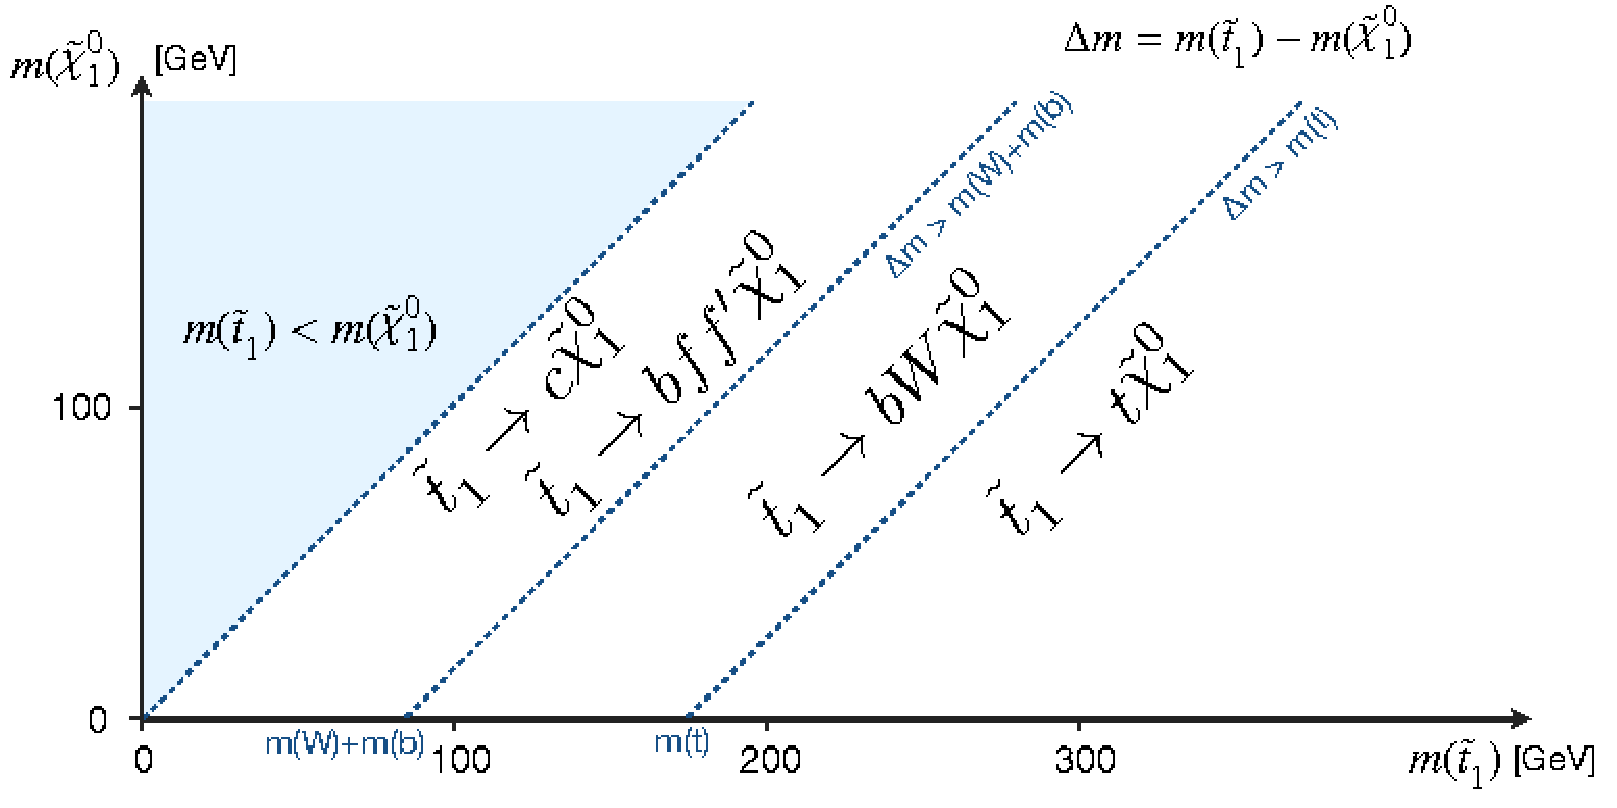
\includegraphics[width=0.75\textwidth]{topSquark_mass_decayModes.pdf}
 	\caption[Top Squark Decay Modes]{Mass parameter space for different decay modes of the top squark.}
 	\label{StopParameterSpace} 
\end{figure}

\begin{table}[!ht]
\begin{center}
\caption[High $\Delta$m Search Regions]{\label{tab:searchregions-hm}Summary of the 130 disjoint search regions that mainly target high \dm~signal models. The high \dm~baseline selection is again $\nj \geq 5$, $\met>250~\GeV$, $\nb\geq1$, and $\dphijonetwothreefour>0.5$.}
\resizebox*{1\textwidth}{!}{

\begin{tabular}{|c|c|c|c|c|c|c|}
	\hline
	\multicolumn{7}{|c|}{$\mtb<175$\,\GeV}  \\
	\hline
	\nj				 & \nb				& \nt			   & \nw				 & \nrt				& \Ht ~[\GeV]		   & \met~[\GeV] 		\\
	\hline
	$\geq7$		& $1, \geq2$  & $\geq0$		 & $\geq0$			& $\geq1$	  & $\geq300$			& $250-300$, $300-400$, $400-500$, $\geq500$ \\
	\hline
	\multicolumn{7}{|c|}{$\mtb\geq175$\,\GeV}  \\
	\hline
	\nj				 & \nb				& \nt			   & \nw				 & \nrt				& \Ht ~[\GeV]		   & \met~[\GeV] 		\\
	\hline
	$\geq5$		& $1,\geq2$   &	$0$				& $0$				   & $0$			 & $\geq1000$		 & $250-350$, $350-450$, $450-550$, $\geq550$ \\
	\hline
	\multirow{6}{*}{$\geq5$} & \multirow{6}{*}{$1$} & $\geq1$ & $0$ & $0$ & $300-1000$, $1000-1500$, $\geq1500$ & $250-550$, $550-650$, $\geq650$\\
						  &					   & $0$			 & $\geq1$			& $0$			  & $300-1300$, $\geq1300$ & $250-350$, $350-450$, $\geq450$ \\
						  &					   & $0$			 & $0$				    & $\geq1$	  & $300-1000$, $1000-1500$, $\geq1500$ & $250-350$, $350-450$, $450-550$, $550-650$, $\geq650$ \\
						  &					   & $\geq1$	 & $\geq1$			& $0$			  & $\geq300$ 			& $250-550$, $\geq550$ \\
						  &					   & $\geq1$	 & $0$					& $\geq1$	  & $\geq300$			& $250-550$, $\geq550$ \\
						  &					   & $0$			 & $\geq1$			& $\geq1$	  & $\geq300$			& $250-550$, $\geq550$ \\
	\hline
	\multirow{10}{*}{$\geq5$} & \multirow{10}{*}{$2$} & $1$ & $0$ & $0$ & $300-1000$, $1000-1500$, $\geq1500$ & $250-550$, $550-650$, $\geq650$\\
						  &					   & $0$			 & $1$					& $0$			& $300-1300$, $\geq1300$ & $250-350$, $350-450$, $\geq450$ \\
						  &					   & $0$			 & $0$				    & $1$	  		& $300-1000$, $1000-1500$, $\geq1500$ & $250-350$, $350-450$, $450-550$, $550-650$, $\geq650$ \\
						  &					   & $1$	 		 & $1$					& $0$			& $\geq300$ 						& $250-550$, $\geq550$ \\
						  &					   & $1$	 		 & $0$					& $1$	  		& $300-1300$, $\geq1300$ & $250-350$, $350-450$, $\geq450$ \\
						  &					   & $0$			 & $1$					& $1$	  		& $\geq300$							& $250-550$, $\geq550$ \\
						  &					   & $2$	 		 & $0$					& $0$			& $\geq300$ 						& $250-450$, $\geq450$ \\
						  &					   & $0$	 		 & $2$					& $0$	  		& $\geq300$ 						& $\geq250$ \\
						  &					   & $0$			 & $0$					& $2$	  		& $300-1300$, $\geq1300$ & $250-450$, $\geq450$ \\
						  &					   & \multicolumn{3}{|c|}{$\nt+\nw+\nrt\geq3$} & $\geq300$ 					   & $\geq250$ \\
	\hline
	\multirow{10}{*}{$\geq5$} & \multirow{10}{*}{$\geq3$} & $1$ & $0$ & $0$ & $300-1000$, $1000-1500$, $\geq1500$ & $250-350$, $350-550$, $\geq550$\\
						  &					   & $0$			 & $1$					& $0$			& $\geq300$ 						& $250-350$, $350-550$, $\geq550$\\
						  &					   & $0$			 & $0$				    & $1$	  		& $300-1000$, $1000-1500$, $\geq1500$ & $250-350$, $350-550$, $\geq550$\\
						  &					   & $1$	 		 & $1$					& $0$			& $\geq300$ 						& $\geq250$ \\
						  &					   & $1$	 		 & $0$					& $1$	  		& $\geq300$ 						& $250-350$, $\geq350$ \\
						  &					   & $0$			 & $1$					& $1$	  		& $\geq300$							& $\geq250$ \\
						  &					   & $2$	 		 & $0$					& $0$			& $\geq300$ 						& $\geq250$ \\
						  &					   & $0$	 		 & $2$					& $0$	  		& $\geq300$ 						& $\geq250$ \\
						  &					   & $0$			 & $0$					& $2$	  		& $\geq300$ 					   & $250-350$, $\geq350$ \\
						  &					   & \multicolumn{3}{|c|}{$\nt+\nw+\nrt\geq3$} & $\geq300$ 					   & $\geq250$ \\
	\hline
\end{tabular}
}
\end{center}
\end{table}

\begin{table}[!ht]
\begin{center}
\caption[Low $\Delta$m Search Regions]{\label{tab:searchregions-lm}Summary of the 53 disjoint search regions that mainly target low \dm~signal models. The low \dm~baseline selection is again $\nj \geq 2$, $\met>250~\GeV$, $\nt=\nw=\nrt=0$, $\nb\geq0$, $\mtb<175~\GeV$ (when applicable), $|\Delta\phi(\text {j}_1,\met)|>0.5, ~~ |\Delta\phi(\text {j}_{2,3},\met)| > 0.15$, $\pt(ISR) > 200$~\GeV, $ |\eta(ISR)| < 2.4$, $|\Delta\phi(j_{\text{ISR}},\met)|>2$, and $\metsig > 10$.}
\resizebox*{1\textwidth}{!}{
\begin{tabular}{|c|c|c|c|c|c|}
	\hline
	$\nj$              & $\nb$                    & $\nsv$             & $\ptisr$~[\GeV]         & $\ptb$~[\GeV]      & $\met$~[\GeV]                           \\
	\hline
	$2-5$              & \multirow{4}{*}{0}       & 0                  & \multirow{4}{*}{$>500$} & \multirow{4}{*}{-} & $450-550$, $550-650$, $650-750$, $>750$ \\
	$\geq6$            &                          & 0                  &                         &                    & $450-550$, $550-650$, $650-750$, $>750$ \\
	$2-5$              &                          & $\geq1$            &                         &                    & $450-550$, $550-650$, $650-750$, $>750$ \\
	$\geq6$            &                          & $\geq1$            &                         &                    & $450-550$, $550-650$, $650-750$, $>750$ \\
	\hline
	\multirow{5}{*}{$\geq2$} & \multirow{5}{*}{1}   & 0                  & $300-500$               & $20-40$            & $300-400$, $400-500$, $500-600$, $>600$ \\
	&                          & 0                  & $300-500$               & $40-70$            & $300-400$, $400-500$, $500-600$, $>600$ \\
	&                          & 0                  & $>500$                  & $20-40$            & $450-550$, $550-650$, $650-750$, $>750$ \\
	&                          & 0                  & $>500$                  & $40-70$            & $450-550$, $550-650$, $650-750$, $>750$ \\
	&                          & $\geq1$            & $>300$                  & $20-40$            & $300-400$, $400-500$, $>500$            \\
	\hline
	$\geq2$            & \multirow{6}{*}{$\geq2$} & \multirow{6}{*}{$\geq0$} & $300-500$               & $40-80$            & $300-400$, $400-500$, $>500$            \\
	$\geq2$            &                          &                          & $300-500$               & $80-140$           & $300-400$, $400-500$, $>500$            \\
	$\geq7$            &                          &                          & $300-500$               & $>140$             & $300-400$, $400-500$, $>500$            \\
	$\geq2$            &                          &                          & $>500$                  & $40-80$            & $450-550$, $550-650$, $>650$            \\
	$\geq2$            &                          &                          & $>500$                  & $80-140$           & $450-550$, $550-650$, $>650$            \\
	$\geq7$            &                          &                          & $>300$                  & $>140$             & $450-550$, $550-650$, $>650$         \\
	\hline
\end{tabular}
}
\end{center}
\end{table}


